\section{Testing and Results}

The testing will be done in two parts: implementation and performance testing.
The implementation testing tests the library implementation result, whether
sensor data can be used and a hardware-in-the-loop simulation can be done. The
performance testing tests, well, the HILS system performance.

\subsection{Testing Environment}

The implementation testing is done on AGX and SILS computers while performance
testing is done on RKB and SILS computer. The specification of RKB and SILS
computers can be seen in Table~\ref{tbl-section-6-computers-specs}. The RKB/AGX
and SILS computers are connected with a 1 Gbps link speed.

\begin{table}[htbp]
	\caption{SILS and RKB Computers Specification}
	\label{tbl-section-6-computers-specs}
	\begin{center}
		\begin{tabular}{r c c}
			\toprule
			                  & CPU & i9-10920X 12C/24T 3.50 GHz \\
			\textbf{SILS}     & RAM & 128 GB                     \\
			\textbf{computer} & GPU & 2x NVIDIA GeForce RTX 3090 \\
			                  & OS  & Ubuntu Linux 20.04         \\
			\midrule
			                  & CPU & i7-8700 6C/12T 3.20 GHz    \\
			\textbf{RKB}      & RAM & 16 GB                      \\
			\textbf{computer} & GPU & NVIDIA GeForce RTX 2070    \\
			                  & OS  & Ubuntu Linux 18.04         \\
			\bottomrule
		\end{tabular}
	\end{center}
\end{table}

\subsection{Implementation Testing}\label{section-4-implementation-testing}

The implementation testing tests the functionality of the library when used in a
running simulation. There are four criterias to be achieved in this category which are

\begin{enumerate}
	\item the speed shown in GRS is the same one from the virtual GNSS sensor,
	\item the camera feed shown in GRS is the same one from the virtual camera
	      sensor,
	\item the lidar images shown in GRS is the same one from the virtual lidar
	      sensor, and
	\item the tram in CARLA can move according to the control sent by GRS.
\end{enumerate}

The result of the implementation can be seen in
Fig.~\ref{fig-section-6-implementation-results}. It can be seen that the camera
feed shown in GRS (right monitor) is the same as the camera window in
ScenarioRunner which is taken from the virtual sensors directly (left monitor).

\begin{figure}[htbp]
	\centerline{\includegraphics[width=0.45\textwidth,trim={12cm 12cm 0 12cm},clip]{resources/chapter-4/HILS-system-running.png}}
	\caption{Implementation Result}
	\label{fig-section-6-implementation-results}
\end{figure}

\subsection{Performance Testing}

The performance testing is done on the RKB and SILS computer. The reason for
using RKB instead of AGX is, during the performance testing period, the AGX
computer was being used for field testing. There are two criterias for this
category:
\begin{enumerate}
	\item CARLA can maintain at least 2 FPS when simulation is running, and
	\item communication latency have to be faster compared to previous HILS
	      system.
\end{enumerate}
The requirement for CARLA to be running with at least 2 FPS comes from project
owner. Furthermore, there's a caveat to testing the second criteria, because the
previous HILS is not up to par in feature and too hard to start, the comparison
is done to a ``theoretical'' version of the previous HILS. The ``theoretical''
version of previous HILS is only implements some operations done in it instead
of the whole process. Moreover, the latency testing only uses GNSS and Camera
sensor. The lidar sensor isn't used because of technical difficulties during the
implementation.

In the performance test, latency is calculated by dividing round-trip time (RTT) by two.
It is calculated in ScenarioRunner/SILS computer side using camera sensor data
and using the formula in Eq.~\ref{eqn-section-6-rtt}.
\begin{equation}
	\label{eqn-section-6-rtt}
	\text{RTT} = T_{e} - T_{s} - t_p
\end{equation}
With:
\begin{table}[!h]
	\begin{tabular}{l l l}
		RTT     & : & round-trip time (in ms)                                  \\
		$T_{e}$ & : & timestamp control is received in ScenarioRunner (in ms)  \\
		$T_{s}$ & : & timestamp first camera segment is sent in ScenarioRunner \\
		        &   & (in ms)                                                  \\
		$t_p$   & : & processing time in GRS (in ms)
	\end{tabular}
\end{table}

$T_e$, $T_s$, and $t_p$ is taken before ZeroMQ library function is called. This
causes a small overhead in the RTT calculation.

The camera data is used to calculate RTT because it has a significantly large
size therefore, the camera data can show the worst case scenario.  Because the
size of the camera data, it can't be transmitted as a single packet using
ZeroMQ, instead it has to be sliced into a smaller segments. The RTT is
calculated from the first segment transmitted so the RTT is the time to send a
sensor data, not the time to send a single segment.

As for the latency calculation in ``theoretical'' previous HILS, it is started
from when the sensor data is sent and until the data is received on the other
side.

The performance testing's results can be seen in
Table~\ref{tbl-section-6-perf-result-statistics} and
Fig.~\ref{fig-section-6-carla-fps}. Using the new HILS implementation, CARLA can
run with 5--13 FPS. Addtionally, the average latency to send camera data is at
least 2.5x faster when compared to the previous HILS.

\begin{table}[!htbp]
	\caption{Performance Testing Statistics}
	\label{tbl-section-6-perf-result-statistics}
	\begin{center}
		\begin{tabular}{c c c}
			\toprule
			                       & Data count   & 1.000     \\
			\cline{2-3}
			                       & Average (ms) & 28,4245   \\
			\cline{2-3}
			                       & Std (ms)     & 4,68      \\
			\cline{2-3}
			\textbf{previous HILS} & Min (ms)     & 16        \\
			\cline{2-3}
			(``theoretical'')      & $Q_1$ (ms)   & 25        \\
			\cline{2-3}
			                       & $Q_2$ (ms)   & 28        \\
			\cline{2-3}
			                       & $Q_3$ (ms)   & 31        \\
			\cline{2-3}
			                       & Max (ms)     & 45,5      \\
			\midrule
			                       & Data count   & 16.891    \\
			\cline{2-3}
			                       & Average (ms) & 10,989965 \\
			\cline{2-3}
			                       & Std (ms)     & 2,248782  \\
			\cline{2-3}
			\textbf{new HILS}      & Min (ms)     & 4,5       \\
			\cline{2-3}
			                       & $Q_1$ (ms)   & 10        \\
			\cline{2-3}
			                       & $Q_2$ (ms)   & 11        \\
			\cline{2-3}
			                       & $Q_3$ (ms)   & 12,5      \\
			\cline{2-3}
			                       & Max (ms)     & 19,5      \\
			\bottomrule
		\end{tabular}
	\end{center}
\end{table}

\begin{figure}[htbp]
	\centerline{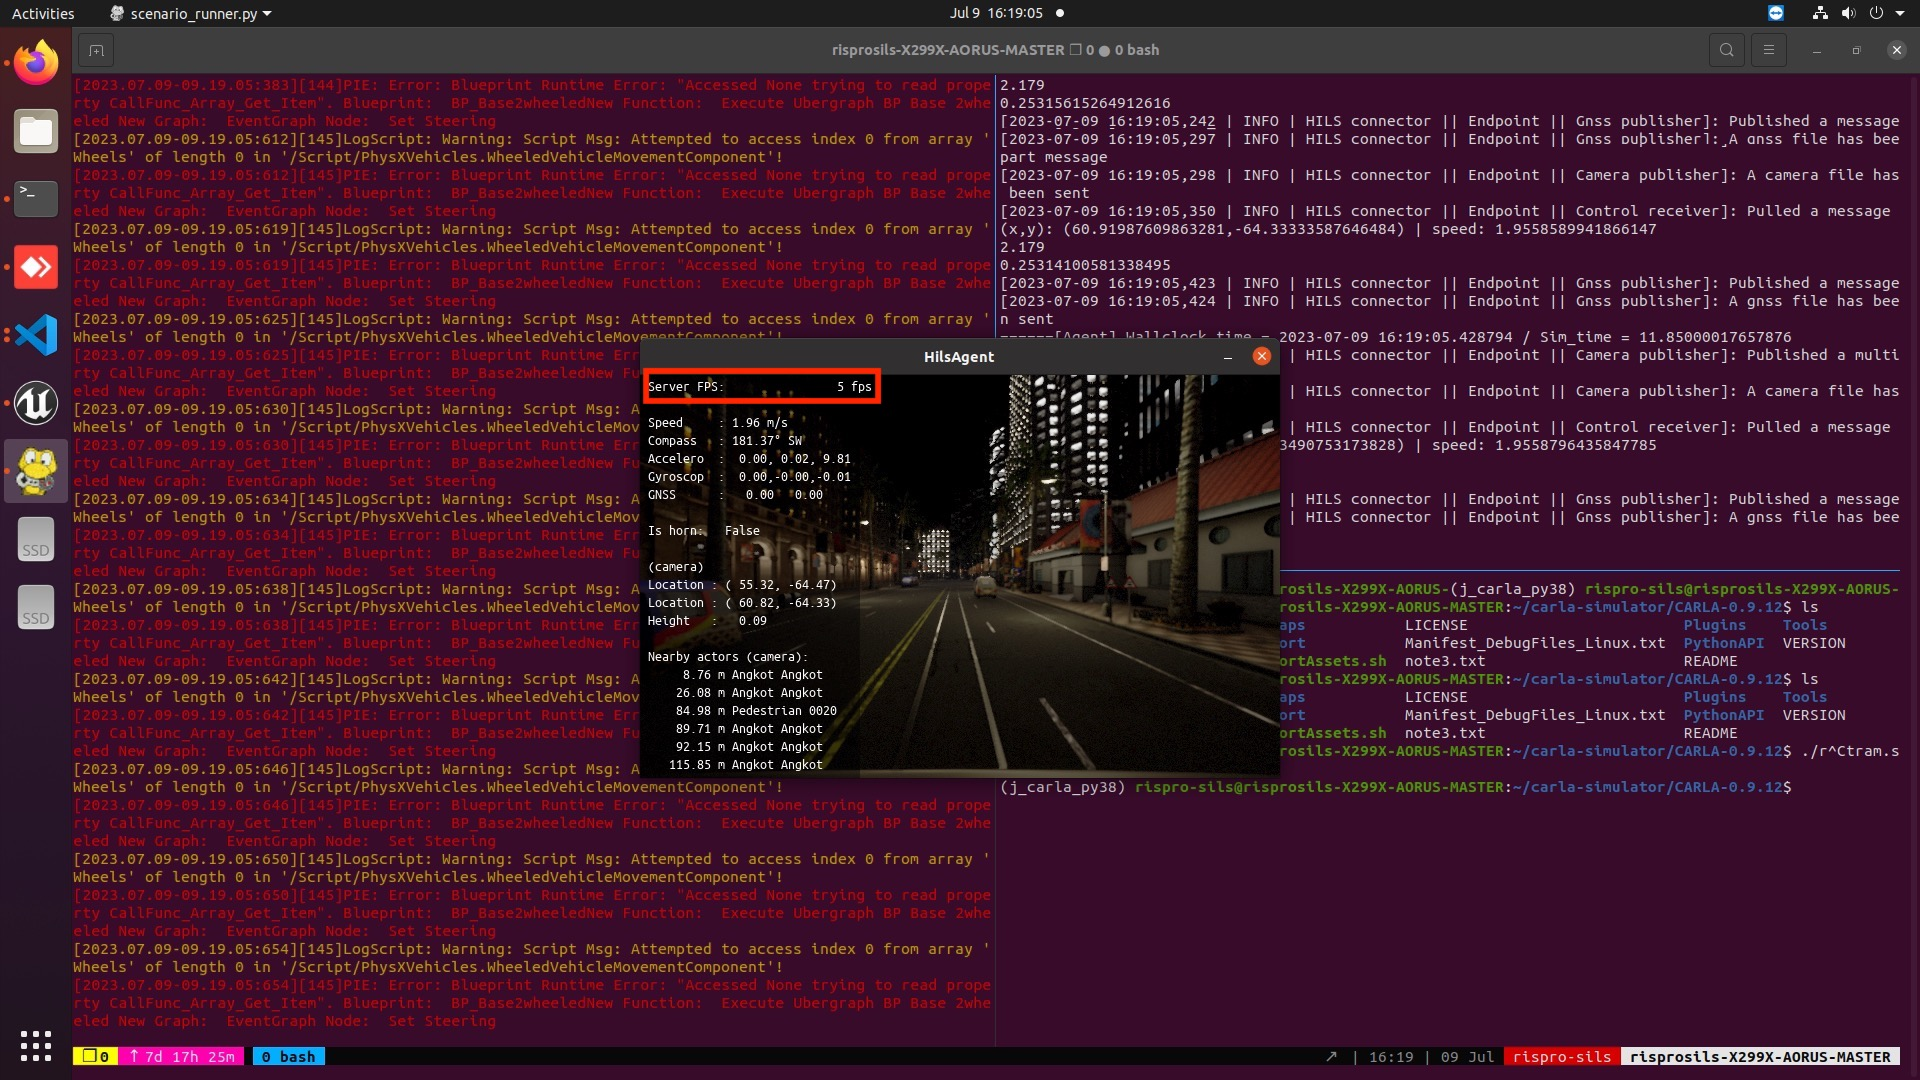
\includegraphics[width=0.45\textwidth,trim={22.5cm 10.5cm 22.5cm 12cm},clip]{resources/chapter-4/CARLA-5FPS.JPG}}
	\centerline{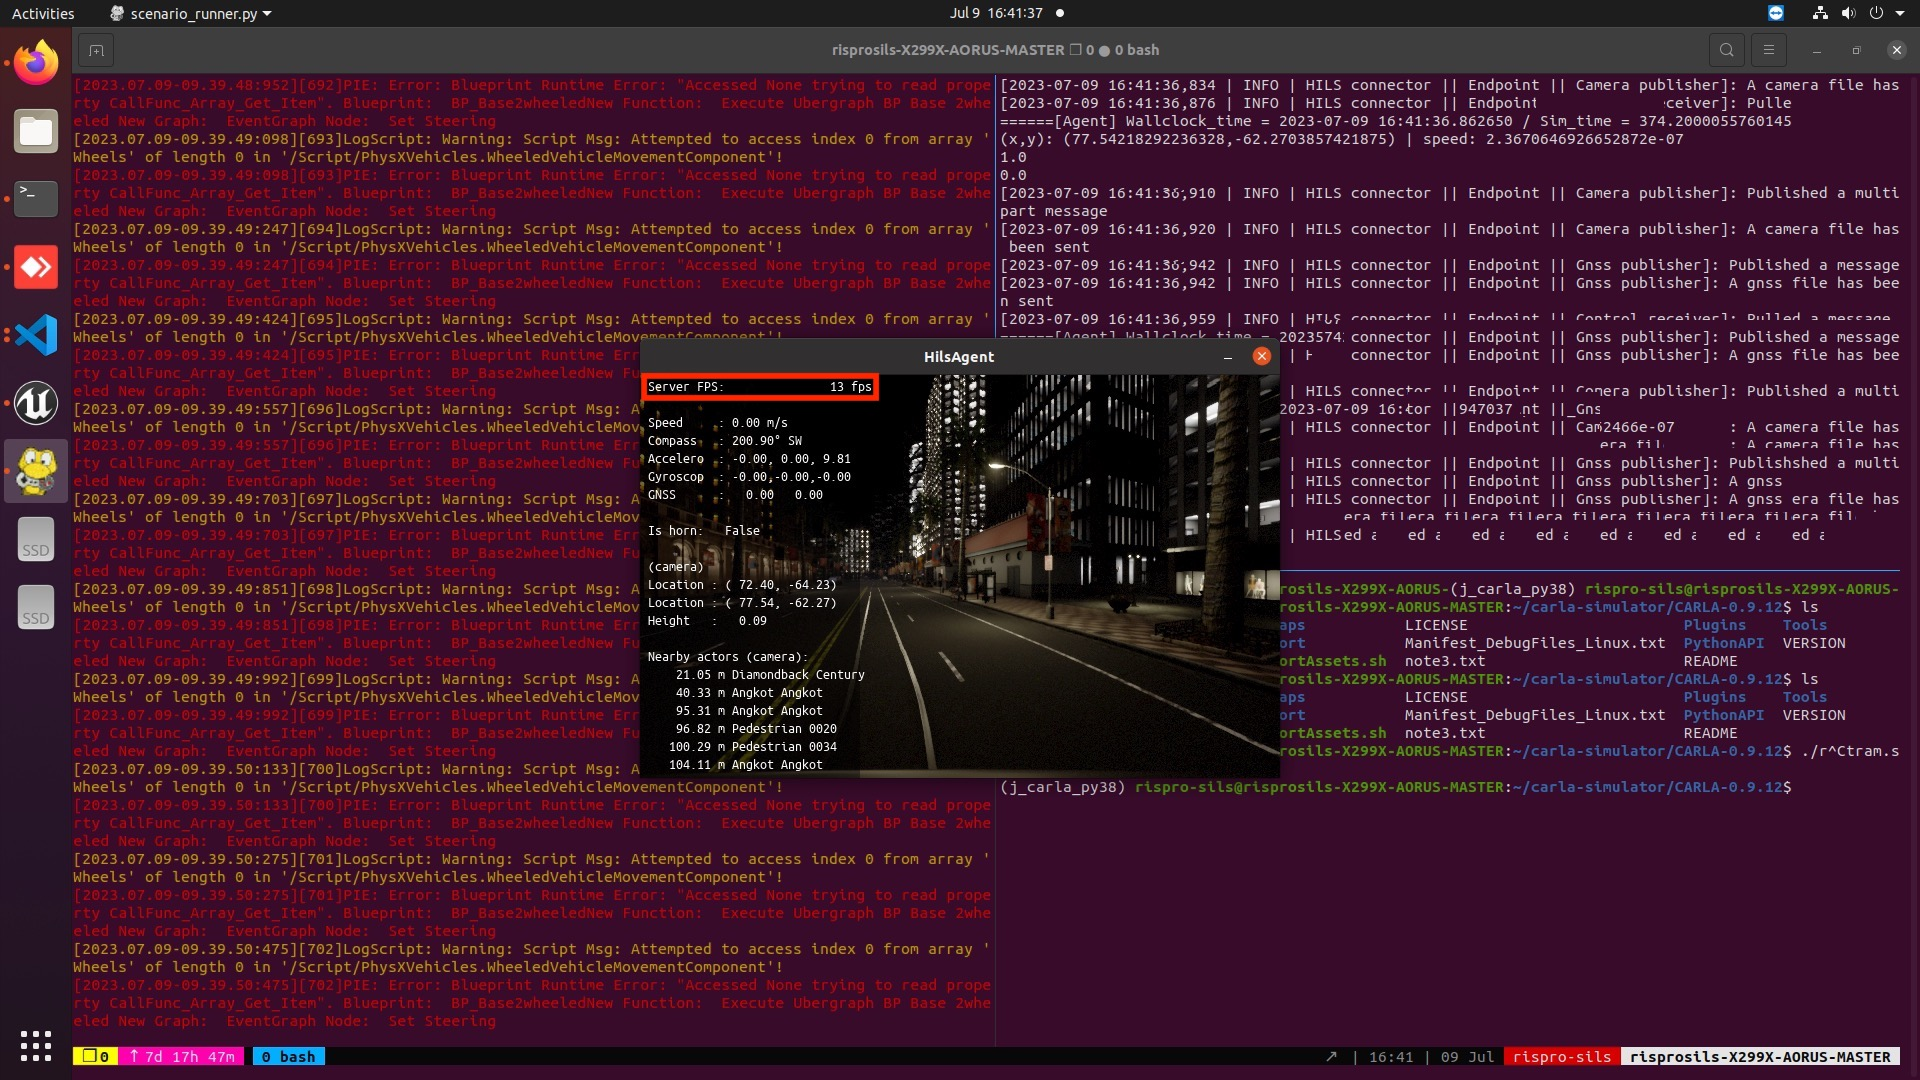
\includegraphics[width=0.45\textwidth,trim={22.5cm 10.5cm 22.5cm 12cm},clip]{resources/chapter-4/CARLA-13FPS.JPG}}
	\caption{CARLA FPS}
	\label{fig-section-6-carla-fps}
\end{figure}